\documentclass[11pt]{article}
\usepackage[margin=1in]{geometry}
\usepackage{fixltx2e}
\usepackage{wrapfig}
\usepackage{graphicx}
\usepackage{url}
\usepackage{hyperref}
\usepackage{fancyhdr}
\usepackage{lastpage}
\date{\vspace{-5ex}}

\title{\bf{DNS Amplification Attack}}
\pagestyle{fancy} 
\fancyhf{}
\lhead{ICTIEE 2014}
\cfoot{Page \thepage  of \pageref{LastPage}}
\date{}
\begin{document}
\maketitle

\newpage
\section*{DNS(Domain Name Server)}
DNS Amplification attack is sophisticated Denial of service attack using DNS server behaviour.So lets disscuss Basics for DNS amplification attack i.e. what is DNS.The Domain Name System (DNS) is a hierarchical decentralized naming system for computers, services, or any resource connected to the Internet or a private network.  It is a Internet Directory Service that uses to store mapping from host name to IP address. Mapping from host name to IP address is called address resolution.It associates various information with domain names assigned to each of the participating entities. Most prominently, it translates more readily memorized domain names to the numerical IP addresses needed for the purpose of locating and identifying computer services and devices with the underlying network protocols. By providing a worldwide, distributed directory service, the Domain Name System is an essential component of the functionality of the Internet.
\\
We use host name Because for communication we need to have IP address but It is very difficult to remember IP address of every host to which you want to communicate. So better solution is to use host name for every host to which you want communicate and for this we require a centralized entity that will store the IP address for the correspoding host name, that centralized entity is Domain Name Server.
\subsection{DNS Working}
Suppose a computer want to visit a site i.e. www.example.com, then in order to visit it we must know its IP address. So computer known as DNS resolver sends a request to DNS server asking for IP of www.example.com. If local DNS has www.example.com 's IP it will return the same otherwise it will ask to one of the root name server , which point to other DNS server. Now DNS resolver send request to other DNS server asking for IP address of example.com. It does so till it get IP address. 
\begin{figure}
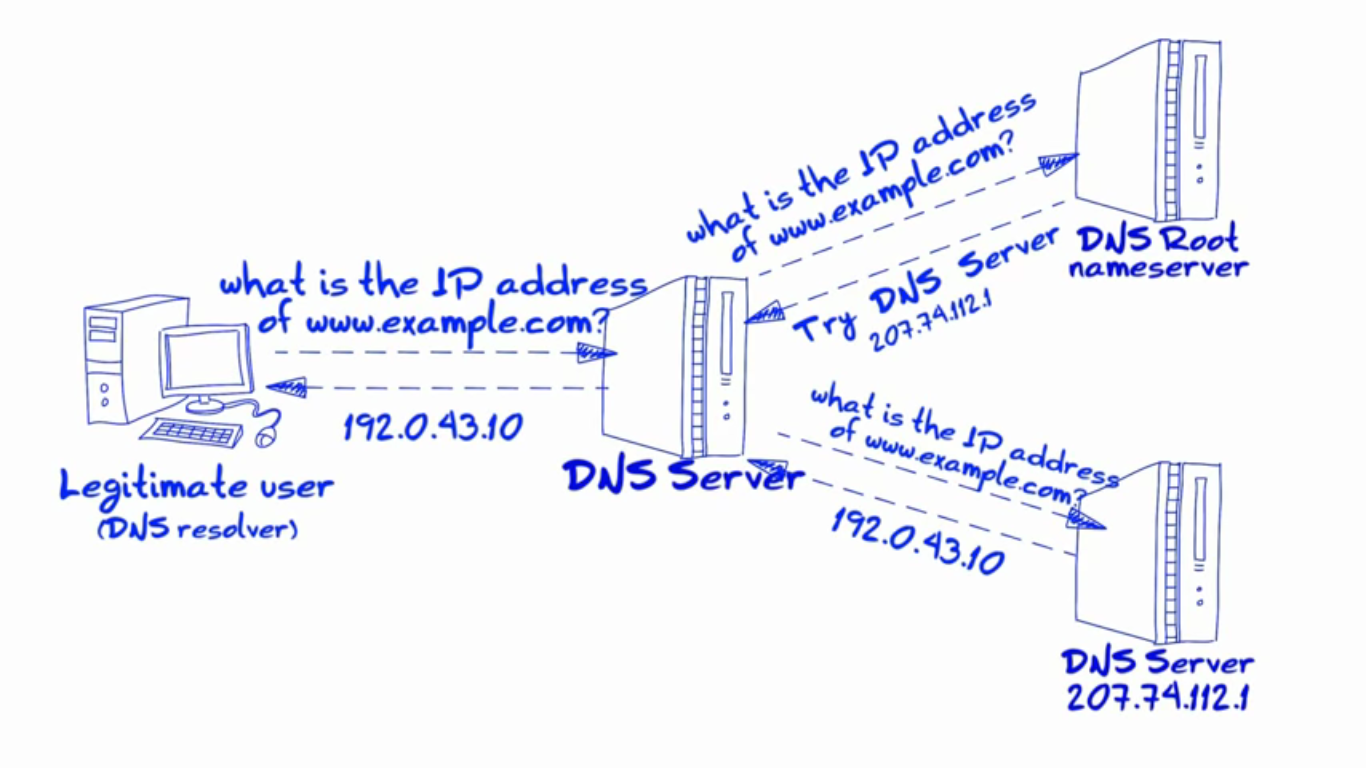
\includegraphics[width=7cm,height=2cm]{pics/dns.png}
\caption{DNS request processing}
\end{figure}

\subsection{Methods to implement DNS}
\subsubsection{Iterative Name Resolution}
In Iterative Name Resolution server tries to resolve the path name as far it can and return every immediate result to the client. Then client if does not get valid ans then it will send request to another DNS Server whose reference is given by previous server's response. \\
Iterative DNS is not vulnerable to DNS amplification attack because in order to execute DNS query using Iterative Name Resolution we need interaction with client. We can complete DNS query without client interaction. So if a attacker spoofs IP of client and sends DNS request to DNS server , but server may not have IP address of requested host name then it will send reference of another DNS server(which is not DNS reply as it is small in size). So now in order to complete the request client need to send request further so attack is not possible in iterative Name Resolution.
\begin{figure}
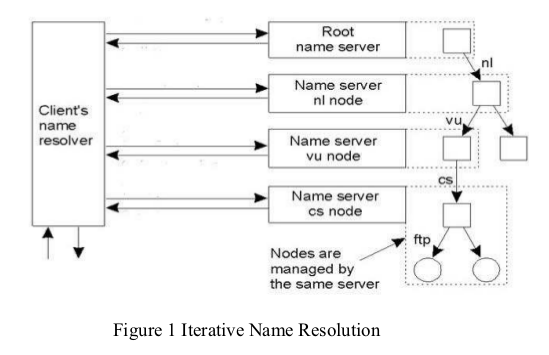
\includegraphics[width=7cm,height=2cm]{pics/iter.png}
\caption{Iterative Name Resolution}
\end{figure}
\subsubsection{Recursive Name Resolution}
In Recursive Name Resolution, server solves the query as far as it can then forward that result to next server to solve the query fully, at the complete result is forwarded to the client. Figure shows the process of the recursive name resolution. 
DNS amplification attack is possible with the Recursive Name Resolution because there is no client interaction in the middle of the processing of the DNS request and client would directly get DNS response. We also attack on the DNS recursive name resolution.
\begin{figure}
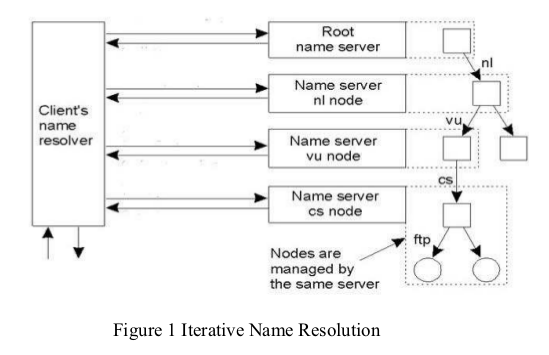
\includegraphics[width=7cm,height=2cm]{pics/iter.png}
\caption{Iterative Name Resolution}
\end{figure}

\section{DOS attack (Denial of Service attack)}
Denial of Service attack is explicit attempt by an attacker to prevent legitimate user from accessing the services (that is supposed to acess by the user).Criminal perpetrators of DoS attacks often target sites or services hosted on high-profile web servers such as banks, credit card payment gateways; but motives of revenge, blackmail or activism can be behind other attacks.
There are many ways in which we can craft DOS attack:
1.Congusting Network Resources : by sending lots of response (DNS reply packet) we can congust the network of the victim.
2.Draining CPU memory : By Syn flood attack we can create lots of half open connection, which allocate memory for these half open connection and eats up the CPU memory.
3.Reducing computing power: victim is busy keep receving and checking checksum and etc of receiving packets , so its computation power got reduce.
4.Poisoning domain name translations : we can make changes in DNS cache by interrupt the response from one server to other server.

\subsubsection{Distributed Denial of Service(DDos)}
this is even more dangerous, in this attacker compromises lots of bots then they will combinedly used to attack victim, that will affect the victim in very less time.Here attack source is more than one, often thousands of, unique IP addresses. It is analogous to a group of people crowding the entry door or gate to a shop or business, and not letting legitimate parties enter into the shop or business, disrupting normal operations.





\end{document}
